\section{Corrections}\label{sec:Corrections}
\subsection{Monte Carlo Embedding Technique}
The correction factors are obtained by the multistep
embedding MC technique. First, simulated tracks are
blended into real events at the raw data level. Real data
events to be used in the embedding are sampled over the
entire data-taking period in order to have proper representation
of the whole data set used in the analysis.  Three samples of embedding MC were produced:
\begin{enumerate}
	\item The MC track kinematics are taken
	from flat distributions in $\eta$ and $p_T$. The flat $p_T$ distribution
	is used in order to have similar statistics in different
	$p_T$ bins.
	\item PYTHIA 8.186 SD  with Sch{\"u}ler and Sj{\"o}strand Pomeron Flux model (\cite{pythia8}).
	\item PYTHIA 8.186 CD  with Minimum Bias Rockefeller Pomeron Flux model (\cite{pythia8}).
\end{enumerate}
The tracks are propagated through the full simulation of
the STAR detector and geometry using GEANT with a
realistic simulation of the STAR-TPC response. The obtained raw data 
information for the simulated particles are added on to
the existing information of the real data. Next, the mixed events are treated just as real data
and are processed through the full reconstruction chain.

\subsection{Data-MC comparison}
\begin{figure}[H]
	\centering
	\parbox{0.484\textwidth}{
		\centering
		\begin{subfigure}[b]{\linewidth}{
				\subcaptionbox{\label{fig:cutFlownpra}}{\includegraphics[width=\linewidth, page=9]{graphics/cutFlow/SDT.pdf}}}
		\end{subfigure}
	}
	\quad
	\parbox{0.484\textwidth}{
		\centering
		\begin{subfigure}[b]{\linewidth}{
				\subcaptionbox{\label{fig:cutFlownprb}}{\includegraphics[width=\linewidth, page=7]{graphics/cutFlow/CPT2.pdf}}}
		\end{subfigure}
	}
	\caption[...]{...}
	\label{fig:cutFlownpr}
\end{figure}
\begin{figure}[H]
	\centering
	\parbox{0.484\textwidth}{
		\centering
		\begin{subfigure}[b]{\linewidth}{
				\subcaptionbox{\label{fig:cutFlowvza}}{\includegraphics[width=\linewidth, page=8]{graphics/cutFlow/SDT.pdf}}}
		\end{subfigure}
	}
	\quad
	\parbox{0.484\textwidth}{
		\centering
		\begin{subfigure}[b]{\linewidth}{
				\subcaptionbox{\label{fig:cutFlowvzb}}{\includegraphics[width=\linewidth, page=6]{graphics/cutFlow/CPT2.pdf}}}
		\end{subfigure}
	}
	\caption[...]{...}
	\label{fig:cutFlowvz}
\end{figure}
\begin{figure}[H]
	\centering
	\parbox{0.484\textwidth}{
		\centering
		\begin{subfigure}[b]{\linewidth}{
				\subcaptionbox{\label{fig:cutFlowEtaa}}{\includegraphics[width=\linewidth, page=2]{graphics/cutFlow/SDT.pdf}}}
		\end{subfigure}
	}
	\quad
	\parbox{0.484\textwidth}{
		\centering
		\begin{subfigure}[b]{\linewidth}{
				\subcaptionbox{\label{fig:cutFlowEtab}}{\includegraphics[width=\linewidth, page=2]{graphics/cutFlow/CPT2.pdf}}}
		\end{subfigure}
	}
	\caption[...]{...}
	\label{fig:cutFlowEta}
\end{figure}
\begin{figure}[H]
	\centering
	\parbox{0.484\textwidth}{
		\centering
		\begin{subfigure}[b]{\linewidth}{
				\subcaptionbox{\label{fig:cutFlowSDetaa}}{\includegraphics[width=\linewidth, page=3]{graphics/cutFlow/SDT.pdf}}}
		\end{subfigure}
	}
	\quad
	\parbox{0.484\textwidth}{
		\centering
		\begin{subfigure}[b]{\linewidth}{
				\subcaptionbox{\label{fig:cutFlowSDetab}}{\includegraphics[width=\linewidth, page=4]{graphics/cutFlow/SDT.pdf}}}
		\end{subfigure}
	}
	\caption[...]{...}
	\label{fig:cutFlowSDeta}
\end{figure}

\begin{figure}[H]
	\centering
	\parbox{0.484\textwidth}{
		\centering
		\begin{subfigure}[b]{\linewidth}{
				\subcaptionbox{\label{fig:cutFlowpta}}{\includegraphics[width=\linewidth, page=5]{graphics/cutFlow/SDT.pdf}}}
		\end{subfigure}
	}
	\quad
	\parbox{0.484\textwidth}{
		\centering
		\begin{subfigure}[b]{\linewidth}{
				\subcaptionbox{\label{fig:cutFlowptb}}{\includegraphics[width=\linewidth, page=3]{graphics/cutFlow/CPT2.pdf}}}
		\end{subfigure}
	}
	\caption[...]{...}
	\label{fig:cutFlowpt}
\end{figure}

\begin{figure}[H]
	\centering
	\parbox{0.484\textwidth}{
		\centering
		\begin{subfigure}[b]{\linewidth}{
				\subcaptionbox{\label{fig:cutFlowdcaa}}{\includegraphics[width=\linewidth, page=6]{graphics/cutFlow/SDT.pdf}}}
		\end{subfigure}
	}
	\quad
	\parbox{0.484\textwidth}{
		\centering
		\begin{subfigure}[b]{\linewidth}{
				\subcaptionbox{\label{fig:cutFlowdcab}}{\includegraphics[width=\linewidth, page=4]{graphics/cutFlow/CPT2.pdf}}}
		\end{subfigure}
	}
	\parbox{0.484\textwidth}{
		\centering
		\begin{subfigure}[b]{\linewidth}{
				\subcaptionbox{\label{fig:cutFlowdcac}}{\includegraphics[width=\linewidth, page=7]{graphics/cutFlow/SDT.pdf}}}
		\end{subfigure}
	}
	\quad
	\parbox{0.484\textwidth}{
		\centering
		\begin{subfigure}[b]{\linewidth}{
				\subcaptionbox{\label{fig:cutFlowdcad}}{\includegraphics[width=\linewidth, page=5]{graphics/cutFlow/CPT2.pdf}}}
		\end{subfigure}
	}	
	\caption[...]{...}
	\label{fig:cutFlowdca}
\end{figure}

\begin{figure}[H]
	\centering
	\parbox{0.484\textwidth}{
		\centering
		\begin{subfigure}[b]{\linewidth}{
				\subcaptionbox{\label{fig:cutFlowhitsa}}{\includegraphics[width=\linewidth, page=10]{graphics/cutFlow/SDT.pdf}}}
		\end{subfigure}
	}
	\quad
	\parbox{0.484\textwidth}{
		\centering
		\begin{subfigure}[b]{\linewidth}{
				\subcaptionbox{\label{fig:cutFlowhitsb}}{\includegraphics[width=\linewidth, page=8]{graphics/cutFlow/CPT2.pdf}}}
		\end{subfigure}
	}
	\parbox{0.484\textwidth}{
		\centering
		\begin{subfigure}[b]{\linewidth}{
				\subcaptionbox{\label{fig:cutFlowhitsc}}{\includegraphics[width=\linewidth, page=11]{graphics/cutFlow/SDT.pdf}}}
		\end{subfigure}
	}
	\quad
	\parbox{0.484\textwidth}{
		\centering
		\begin{subfigure}[b]{\linewidth}{
				\subcaptionbox{\label{fig:cutFlowhitsd}}{\includegraphics[width=\linewidth, page=9]{graphics/cutFlow/CPT2.pdf}}}
		\end{subfigure}
	}	
	\caption[...]{...}
	\label{fig:cutFlowhits}
\end{figure}

\subsection{Vertex reconstruction}
In $pp$ collisions, where the charged-particle multiplicity is low, the vertex finding algorithm sometimes fails to find a primary vertex. In addition, at high luminosity, vertex finder can fail due to the contribution of pile-up events and providing a wrong reconstructed vertex. In this study we require at least two reconstructed global tracks $N^{global}_{reco}\geq 2$ passing all the quality cuts listed in Table \ref{tab:trackCut} but without $\textrm{DCA}_{xy}$ and $\textrm{DCA}_{z}$ cuts. 

\subsubsection{Track quality cuts used for vertexing}
The tracks used by vertex finder have to  pass different set of quality cuts than used in this analysis. 
A global track $N^{global}_{vrt}$ used in vertex reconstruction has to pass the quality cuts listed in the Table \ref{tab:trackCutVertex}. Since that, vertex reconstruction efficiency and fake vertex rate is calculated as a function of $N^{global}_{vrt}$ instead of $N^{global}_{reco}$. 


\begin{table}[H]
	\centering
	\begin{tabular}{| l | l |}
		\hline			
		Quantity & Cut \\
		\hline
		\hline
		Number of Fit Points & Fit Points $>20$\\
		Transverse Impact Parameter & $|d_0|<2$~cm\\ 
		Ratio of Fit Points / Possible Fit Points & Fit Points/ Possible Fit Points $>0.52$\\
		Global Track Transverse Momentum & $p_{T}>0.2$~GeV/c\\
		TOF Matched Track & TOF Match-Flag $\geq1$\\
		\hline  
	\end{tabular}
	\caption[Vertexing Track Level Cuts]{Vertexing Track Level Cuts}
	\label{tab:trackCutVertex}
\end{table}
\subsubsection{Vertex efficiency and fake vertex}
